\documentclass{article}

\usepackage{graphicx,epstopdf}
\usepackage[hyphens]{url}
\usepackage{color}
\usepackage{indentfirst}
\usepackage{multirow}
\usepackage{rotating}
\usepackage{pifont}

\newcommand{\etal}{{\it et. al.}}
\newcommand{\blue}[1]{\textcolor{blue}{#1}}
\newcommand{\red}[1]{\textcolor{red}{#1}}
\newcommand{\green}[1]{\textcolor{green}{#1}}
\newcommand{\cmark}{\ding{51}}%
\newcommand{\xmark}{\ding{55}}%
\begin{document}

%\section{Introduction}
Online video streaming is the most popular service on the Internet. The pervasive penetration of smartphones and the availability of cheap LTE networks make it even easier to reach millions of users. Video streaming can be primarily categorized into three categories: i) static video or video-on-demand (VoD) streaming, ii) live video streaming, and iii) interactive video streaming. Video streaming services like YouTube, NetFlix, Prime videos fall into the video-on-demand category. Here the videos are prerecorded and preprocessed. YouTube-Live, Periscope, Twitch provide services of live video streaming Category. From a player's perspective, the only difference between VoD and live video streaming is that the videos are not preprocessed in live streaming as it is not ready yet. The services like video conferencing, webinars fall into the third category, the interactive video. The interactive online videos are not only bidirectional but also extremely delay-sensitive. Unlike VoD or live streaming, it is okay for interactive video streaming to drop several frames than stall for data. So, the technologies required for interactive videos are very different in every aspect. In our work, we concentrate on the VoD and live video streaming over HTTP only.

HTTP is a widely accepted protocol as it serves the World-Wide-Web (WWW). Most of the firewalls, proxies, and NAT-boxes allow HTTP protocol. HTTPS, the secure version of HTTP, is equally acceptable for the network administrator of different organizations. So, the HTTP(S) based video streaming services also allowed by those firewalls, proxies, and NAT boxes. This one feature increases the popularity of HTTP(S) based video streaming over the existing video streaming system.

On top of the HTTP-based video streaming system, service providers can adapt video quality according to the available network quality using technology like MPEG-DASH (Dynamic Adaptive Streaming over HTTP), Apple's HLS, or Microsoft's SmoothStreamin. These technologies reduce the rebuffering significantly. Currently, most online video services support adaptive video streaming as it provides a better quality of experience to the viewers. Although different organizations develop these technologies, they work almost identically. In our work, we concentrate on the DASH only as it is a guideline than a product and the open-source implementation of DASH is available.

DASH or DASH-like video streaming systems change video quality on the fly by running a special algorithm call adaptive bitrate (ABR) algorithm. The selection of ABR is crucial as the overall quality of experience is dependent on the ABR algorithm. It is the ABR algorithms' job to provide minimal rebuffering while maintaining better video quality. In this chapter, we discuss the details of the DASH and the different components of DASH.  We then discuss the latest research on the ABR to improve QoE for both VoD and live streaming in different scenarios and conclude with the available research scope.



\section{Dynamic Adaptive Streaming over HTTP}
\begin{figure}[!t]
	\centering
	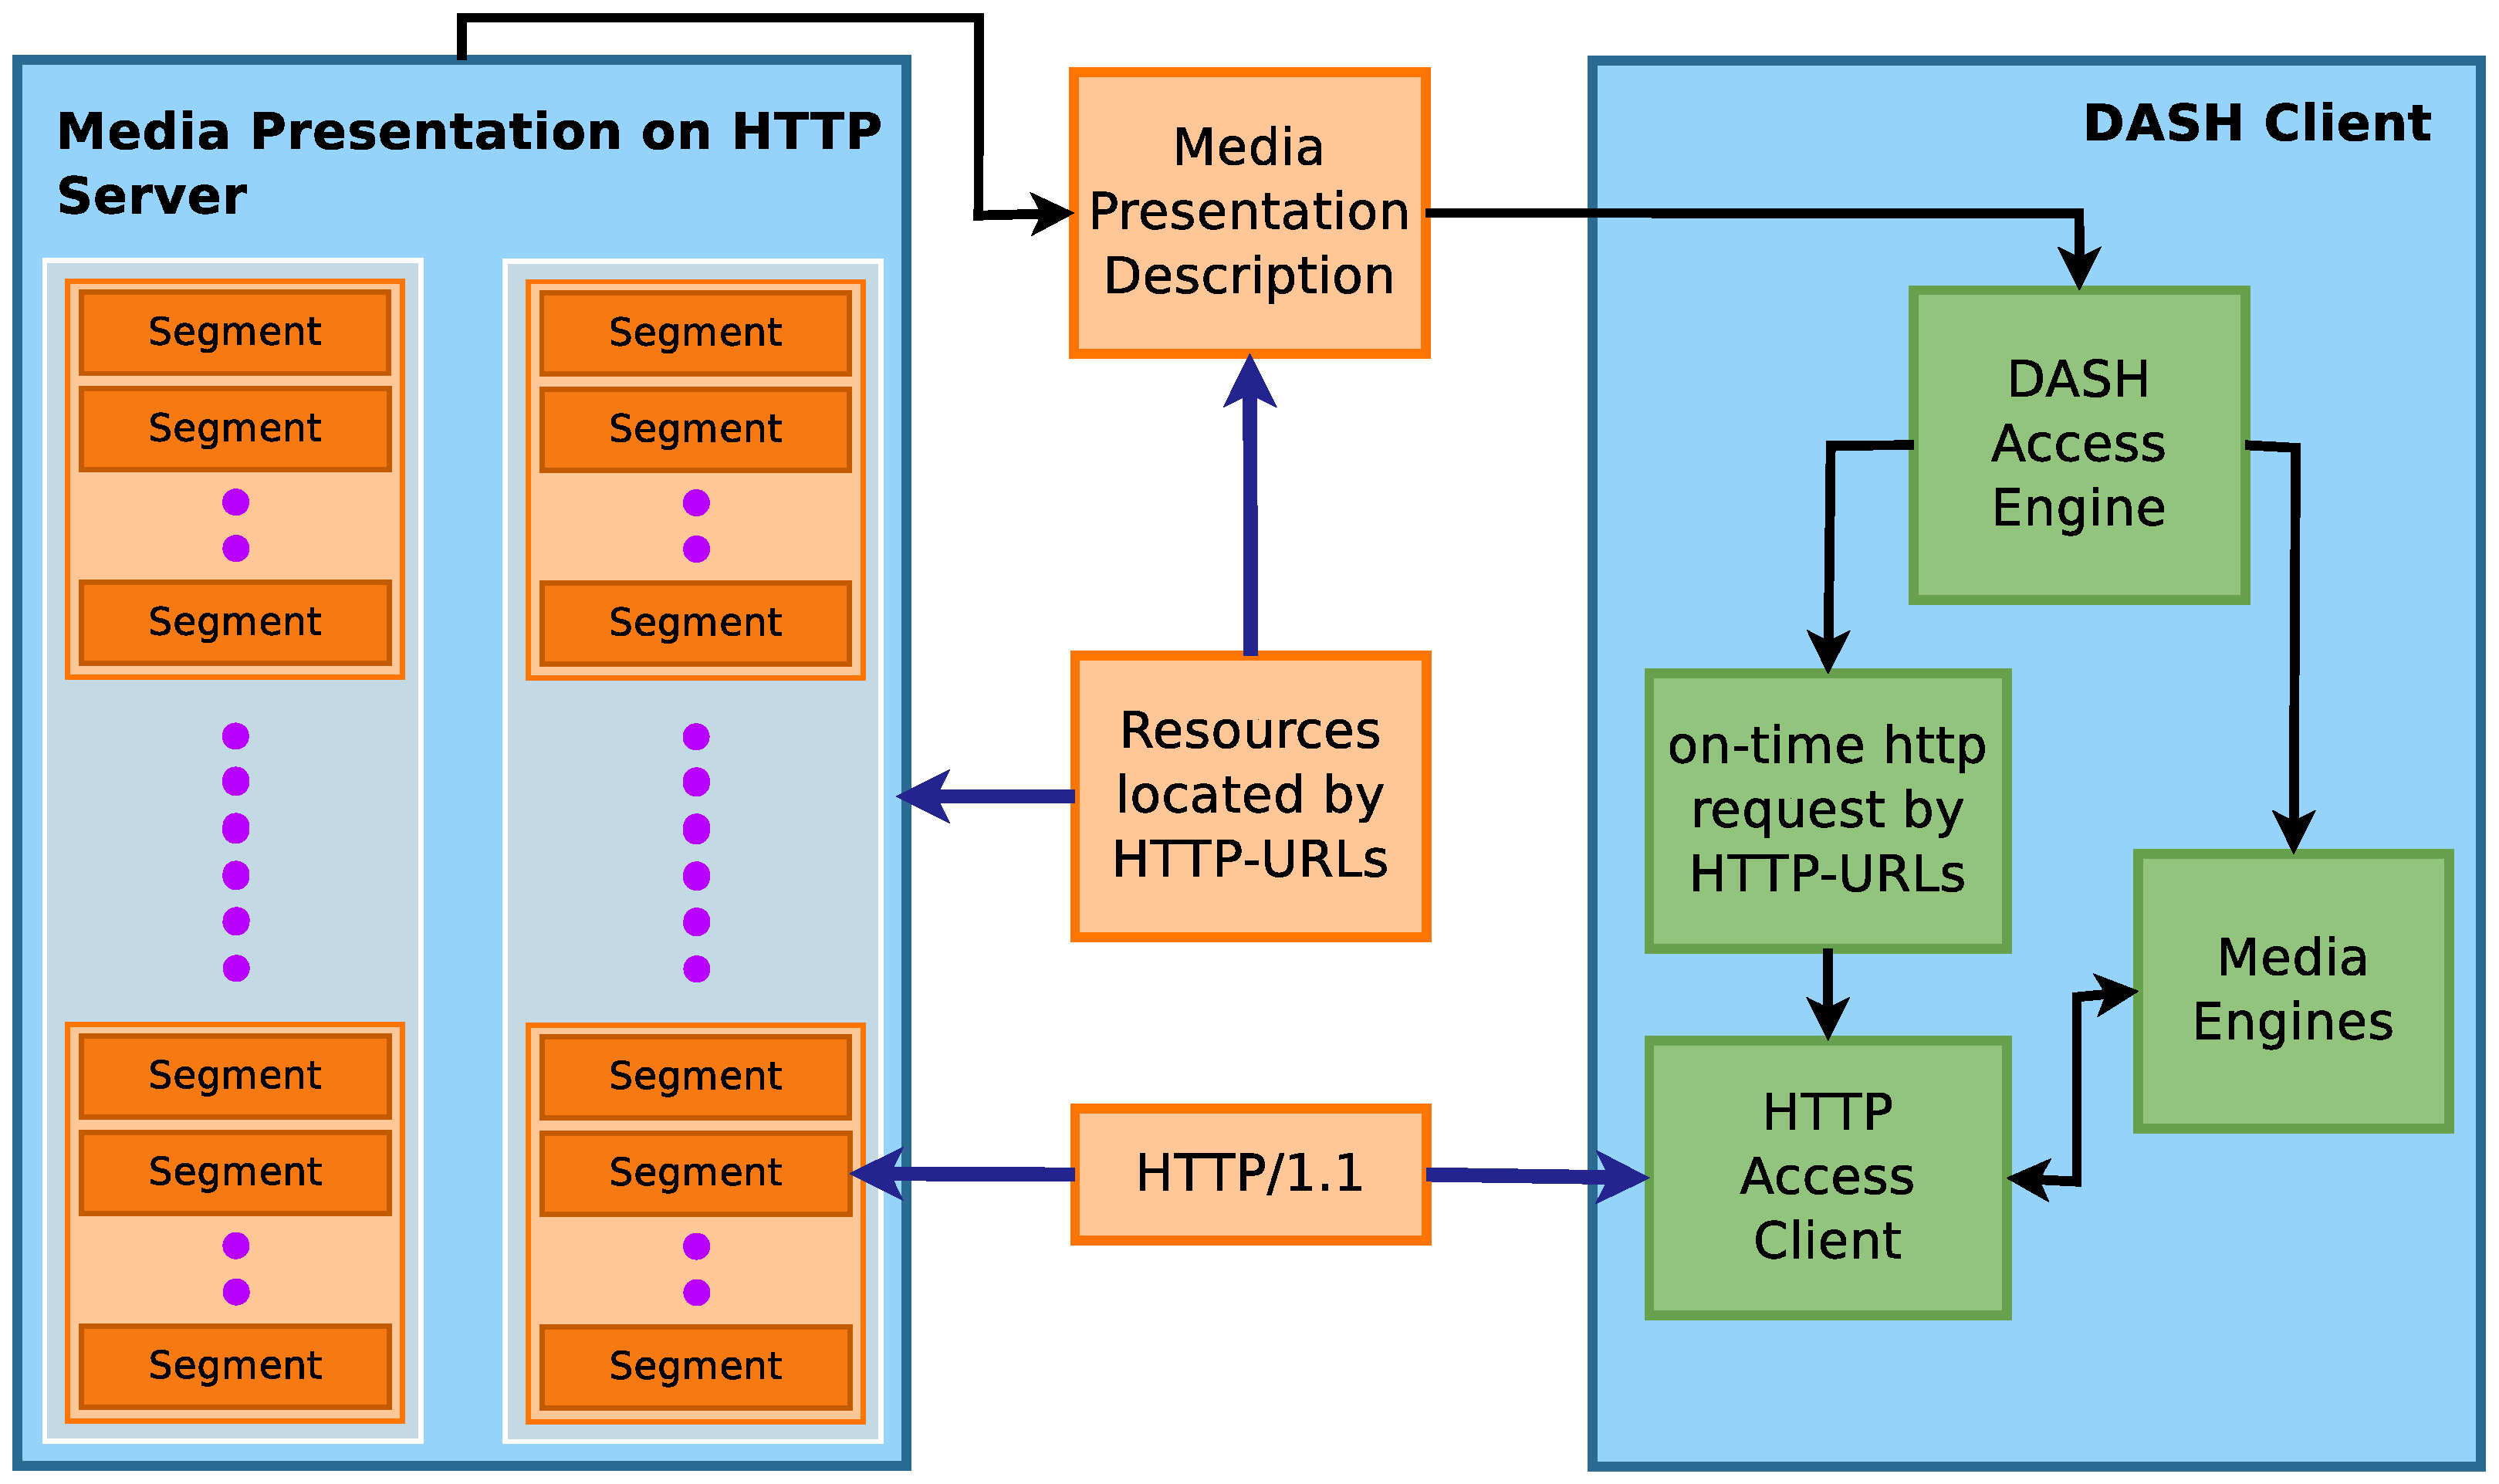
\includegraphics[scale=0.15]{img/dash-arch}
	\caption{\small{DASH Architecture -- On the left side, the server-side media storage is shown, where content is divided into small segments of alternative bit-rates. On the right side, the DASH client architecture is shown; the {\it DASH Access Engine} monitors network bandwidth at the client and accordingly decides which segment to request from the server. (Image Source: https://www.w3.org/2011/09/webtv/slides/W3C-Workshop.pdf)}}
	\label{fig:dash}
\end{figure}
In 2009, Apple developed the HTTP Live Streaming to replace the existing RTSP based streaming for its QuickTime live streaming server\footnote{\url{https://appleinsider.com/articles/09/07/08/apple_launches_http_live_streaming_standard_in_iphone_3_0.html} (accessed: \today)}. Dynamic Adaptive Streaming over HTTP (DASH), sometimes calls as MPEG-DASH, is a technology developed under MPEG to stream video over HTTP. MPEG started working for DASH in 2010 and standardized in 2011\cite{ISO/IEC23009-1:2019}. After the release of {\tt dash.js} by DASH Industry Forum (DASH-IF), almost all the streaming services, including YouTube, NetFlix, Samsung, adopted the DASH in their services.

Video streaming using DASH is a two-step procedure: a) preprocessing video files to distribute and b) the streaming. In the preprocessing (we also call it DASHifying), the streaming provider needs to create the video's required files. It first split the audio and video stream and encode them into multiple bitrate variations. At this phase, the encoder needs to ensure that it aligns the I-frames \footnote{I-frame: a special type of frame that contains a complete picture and no-other frame required to render it. More details: \url{https://en.wikipedia.org/wiki/Video_compression_picture_types}} across different bitrate versions and place all the metadata at the beginning of the file. After encoding, three different types of files are created from the streams. These files are, i) media index files, ii) media data files, and iii) a media presentation description file.

{\bf Media index files:} In general, when any media data stored in a file, the file contain two pieces of information, a) the initialization part and b) the encoded media data. The initialization part contains information to decode the encoded data, which is a kind of index for the original media data. The DASH mandate that this initialization data should store in a separate file. So, while encoding video into different bitrate variation, the metadata part needs to be kept at the output file's beginning. The index files are usually smaller than any of the Media data, so it does not pose any overhead to the system.

{\bf Media data files:} The media data file contains the encoded media. According to DASH, media data are segmented in multiple chunks with equal playback time. All the segments should have an I-frame  at the beginning of the chunk.

{\bf Media presentation description:} It is a {\tt XML} file that contains the metadata required to stream the video. It lists the different audio and video quality available for stream and the URLs for the media index and media data. It also contains the codec, bitrate, and playback duration of individual chunks for each quality.

The preprocessing phase ends with placing all these different files in an HTTP(S) file server. DASH does not require anything else on the server-side to stream a video. It is valid for VoD as well as Live streaming. However, in live streaming, the segments need to be created on the fly and place in the server before any client requests it.

The second phase of the DASH based streaming is streaming the video. DASH requires a smart player that can understand the DASH and play the video. Whenever a player wants to play the DASH based video streaming, it first has to download the MPD file and read it to get other information regarding the stream. The player then has to decide which quality it wants to play based on the ABR algorithm running inside the player and get the preferred quality's chunk accordingly. DASH offloads the entire decision to the player so that any existing content delivery network can stream video content. There are instances where media index files and media data are not chunked instead kept in a fixed file. While this saved lot of disk space, the server have to support the HTTP range-request\footnote{\url{https://developer.mozilla.org/en-US/docs/Web/HTTP/Range_requests}}, and the player can get the desired chunk using the {\tt range} header.

DASH also allows streaming providers to support various client platforms and encode video in various codec and put all the information in the MPD file. Although the MPD file can get very big, the player can choose a platform supported codec and play it without any hassle.


\subsection{Adaptive Bitrate Algorithm}
The adaptive bitrate algorithm is the heart of the DASH based streaming system as it decide the quality of each and every segment on the fly. By default, ABR algorithm runs just before fetching the next chunk. As ABR algorithm is part of the player, it have access to all the playback related parameters and it can use any of those parameter to decide quality for next chunk. The primary goal of any ABR algorithm is to maximize to QoE which is combination of three parameters:
\begin{itemize}
	\item {\bf Quality:} Quality of video or audio is determined by the sharpness of the video. Sharpness of a video is directly related to the bitrate of sharpness increases. It is expected that sharp media have better details in the media in both audio and video thus provide better experience in enjoying the stream. Any ABR tries to maintain bitrate as high as possible so that the quality of experience improves.
	\item {\bf Smoothness:} DASH allows player to change video quality on the fly. Frequent quality change disrupt the smoothness of the video watching experience. So, ABR need to minimize the quality change during playback.
	\item {\bf Rebuffering:} Rebuffering is the most irritating experience for any user. The entire DASH and DASH like system is developed just to minimize rebuffering. It outmost responsibility of any ABR to minimize the rebuffering by selecting appropriate quality based of the current network quality.
\end{itemize}

The ABR algorithms are part of the DASH based streaming client. Any player have to implement at least one ABR algorithm in there implementation to support the quality adaptation.

The penetration of the smartphone and wide access to 4G-LTE cellular data is one of the many reason behind the popularity of DASH based streaming. All the major smartphone provide API to build DASH based streaming client using native player. Most of the smartphones also support HTML5 enable webview using which DASH based player can be developed at ease.

\subsection{HTML5 and DASH}
The world wide web consortium (W3C) specifies the experimental media source extension (MSE) which allow JavaScript to manuplate HTML5 video player directly. It also allows to push byte-stream of media data directly to the player decoder and change the player buffer as per requirement on-the-fly. The MSE provide a rich set of API which is being used to developed DASH based video streaming client as all the major browser support the MSE. With introduction of MSE, providing video streaming service become easier as no fancy player need to be installed in the user end and it become easier to update the player just by changing the {\tt JavaScript} player library.


\section{Classical Adaptive Bitrate (ABR) Algorithm}
There are many classical ABR algorithms designed from the inception of DASH based video streaming. Any classical ABR algorithm's primary goal is to run on a low-powered device and not require any learning model. The classical ABR algorithms can be further categorized in {\tt buffer based}, {\tt throughput based}, {\tt hybrid} ABRs. We discuss a few ABR algorithms from each category in this section.

\subsection{Throughput based ABR algorithm}
Any ABR's primary job is to play video without rebuffering. To achieve this simple task, initially, ABR algorithms used to start with the lowest bitrate to quickly start the video and improve quality in subsequent segment until it detects some congestion or loss \cite{5677508,10.1145/1943552.1943575}. While this technique avoids rebuffering, it changes video quality for almost all the segment. Microsoft starts using a little more conservative solution in \cite{10.1145/1943552.1943574} while adapting bitrate based on the network quality. These algorithms have mitigated the rebuffering by matching the video bitrate with the observer network bitrate. However, they have failed to consider the fact that frequent change in quality can be an issue. These algorithms have the goal to improve the average quality and reduce the rebuffering. Later on, the ABR algorithms are designed to maintain the QoE. Few such algorithms are:

\subsubsection{QoE aware DASH (QDASH)}
Mok \etal\ design the QDASH\cite{10.1145/2155555.2155558}, one of the early ABR algorithms with the awareness of QoE, consider that the abrupt quality change is not acceptable. The algorithm has two parts, a) ABR algorithm and b) Bandwidth measurement tool. They proposed a particular module to run at the streaming server, which measures the client bandwidth. The ABR algorithm explicitly connects the measurement module and get in the bandwidth information. With the bandwidth information, QDASH finds the most suitable bitrate. However, QDASH does not switch to the most suitable bitrate immediately. Instead, it switches to the next bitrate to increase the QoE.

\subsubsection{Fair, Efficient, and Stable adapTIVE (FESTIVE)}
FESTIVE\cite{10.1145/2413176.2413189} is a DASH based video streaming system that provides fairness between players that share bottleneck stably and efficiently. Jiang \etal\ show that the measured throughput may not be correct, and the available bottleneck bandwidth might be underutilized due to the scheduling scheme. So, they suggested a method, including three steps. These steps are:\\
a) Estimate the available bandwidth as the harmonic mean of the last 20 throughput measurements.\\
b) Never to jump bitrate, increment or decrement should not go beyond 1 level. \\
c) Randomized the segment scheduling so that all the players get a fair share of the bottle link.

\subsubsection{FEedback Linearization Adaptive STreamIng Controller (ELASTIC)}
All the client-side adaptive algorithms generate an on-off traffic pattern, which leads to unfairness among the players. Cicco \etal\ designed ELASTIC\cite{6691442}, a client-side controller that does not generate on-off traffic pattern. ELASTIC select video bitrate for a segment in such a way so that it finishes downloading the segment at the time when the next segment needs to be downloaded. So, there is no requirement for the on-off traffic generation, and traffic can be fair as underlying TCP is fair for the long-running system.

\subsubsection{Presto}
Zhang \etal\ designed Presto\cite{7249417}, which provides fairness among the players that stream video from multiple servers. They argue that a player might consume more bandwidth of the bottleneck by running more parallel flows. So, they provide a mechanism to restrict a player's bitrate with more flows and improve quality. Presto exploits the fact that a user gets annoyed with drastic bitrate drop; however, not with drastic bitrate increase\cite{10.1145/2018602.2018611}. It also suspends some flows to stabilize the bandwidth utilization for the time and resume later.

\subsubsection{Spectrum-based QUality ADaptation (SQUAD)}
SQUAD\cite{10.1145/2910017.2910593} is a spectrum\cite{1386243} based quality adaptation technique for DASH based video streaming system. Wang \etal\ assumes spectrum as the variation in the bitrate around some $N$ number of segments. The proposed system starts with providing a new method to measure the throughput. Typically throughput is measured when segments have been downloaded, and estimations are made based on the past throughput measurement. The authors have pointed out that this technique may not be correct as the sizes of the segments are different, and thus it might take different times to download different segments even if the bandwidth and bitrate are the same. So, SQUAD suggested performing a running average of throughput over the course of the segment downloading. It proposed to set the bitrate of a few initial segments to the lowest bitrate available and, after the initial set of segments, set bitrate in such a way so that the bitrate variation in a window, i.e., SPECTRUM, is the lowest.


\subsection{Buffer Based}
The buffer-based bitrate adaptation technique is an alternative technique of throughput based where the player does not need to estimate the throughput to adapt the playback quality as the throughput estimation is complex and most of the time inaccurate due to the nature of network dynamics. Also, middleboxes like catching devices, including proxy, make it more difficult to estimate real throughput. Buffer-based ABR algorithms do not suffer from a similar problem. In the past decade, researchers have designed several buffers based ABR algorithms. We are going to discuss a few of those algorithms.

\subsubsection{Buffer based rate adaption}
Huang \etal\ (\cite{Huang2014,10.1145/2398776.2398800,10.1145/2491172.2491179}) describe a bitrate adaptation mechanism solely based on the playback buffer level. The author suggested that the playback buffer is a function of bitrate and network throughput. Thus player buffer level can be an indication of whether to change bitrate or not. Authors use a rate to buffer map to calculate the bitrate for a given buffer. They use an algorithm to remove any fine boundary between bitrates to avoid frequent bitrate fluctuations.

\subsubsection{Threshold driven buffer based adaptation}
Miller \etal\ design a buffer based algorithm in \cite{6229732} as an remedy for the measurement problem of througput driven algorithms. They uses 3 buffer levels $B_{min}$, $B_{low}$ and $B_{max}$ ($0 < B_{min} < B_{low} < B_{max}$) as threshold to decide the bitrate switch. The algorithm aims to keep the buffer level to close to mean of $B_{low}$ and $B_{max}$. It decrease the bitrate if buffer level goes below $B_{low}$, drops to lowest if it goes below $B_{min}$ and increase if it goes beyond $B_{max}$.

\subsubsection{Smooth Adaptive Bit RatE (SABRE)}
SABRE is designed to mitigate the buffer bloat effect of TCP, which might cause queuing delay up to a few seconds in case of HTTP streaming. Mansy \etal(\cite{10.1145/2483977.2484004}) suggested using the HTTP pipeline where multiple HTTP-request can be pushed together. At the client-side, make {\tt recv} call in a non-aggressive way to reduce the queuing delay. Due to its paced {\tt recv} call, it is impossible to measure throughput correctly. So, it changes the pacing of {\tt recv} call based on the playback buffer. The player changes the bitrate as per the observed download rate, which is governed by the non-aggressive pacing.

\subsubsection{Buffer Occupancy based Lyapunov Algorithm (BOLA)}
BOLA\cite{Spiteri2016} treat ABR streaming as an optimization problem where the average bitrate needs to maximize, and rebuffering needs to be minimized. Spiteri \etal\ solves the problem using Lyapunov optimization and provides a theoretical guarantee on the QoE. BOLA does not require any estimation of the throughput. Instead, it is solely based on the playout buffer.

\subsubsection{Adaptation \& Buffer Management Algorithm (ABMA+)}
Beben \etal\ proposes ABMA+\cite{10.1145/2910017.2910596} which predicts the video freezing probability for each representation and selects the best representation satisfies the predefined freezing probability threshold. It continuously monitors the segment download time and uses time characteristics, and the precomputed buffer-map decides the best bitrate for smooth playback.

\subsubsection{Markov Decision-Based Rate Adaptation Approach (mDASH)}
mDASH\cite{7393865} formulate rate adaptation problem as Markov Decision Process (MDP)\cite{P-1066} optimization. According to Zhou \etal\, the state vector define the system state, including buffer occupancy, playback rate, previous video bitrate, network bandwidth. The action is the bitrate for the next segment. They calculate reward based on various parameters that affect the visual quality, including quality, quality switch frequency and magnitude, and rebuffering. The optimization problem is difficult to solve directly as there are many uncertainties during the streaming session due to time-varying network conditions, so the authors proposed a sub-optimal greedy solution to solve the problem. According to their evaluation mDASH perform at per with the optimal solution.

\subsection{Hybrid ABR algorithms}
Some ABR algorithms consider both buffer and throughput to adapt the bitrate. These algorithms can be further categorized in control system based and without control system based. We will discuss few of them here.

\subsubsection{Smooth rate adaptation}
The authors of \cite{10.1145/2413176.2413190} and \cite{6694183} proposes a method involving a control loop and measured throughput and playback buffer. The control loops start with a playback buffer and a reference buffer, and the difference between these two is used to predict the throughput. Then the predicted throughput is used to determine the video bitrate. The video bitrate and the real throughput lead to playback buffer occupancy, further used in the control loop.

\subsubsection{Probe and Adapt (Panda)}
Li \etal\ (\cite{140405}) found that most of the widely deployed DASH like streaming suffers from bitrate fluctuation when multiple players share a bottleneck. They also found that the fluctuation depends on various parameters, including the number of players, players' start time, and background traffic. While digging more, they found that all the techniques assume that the measured throughput is fair and directly used. However, it is not true and due to this fundamental mistake player lost the capability of over-coming buffer underrun. Li \etal\ suggested using probe the network to find the available bandwidth. PANDA uses TCP like the AIMD scheme for rate-adaptation. However, it only uses the probe per chunk instead of per RTT.

\subsubsection{Segment Aware Rate Adaptation (SARA)}
SARA\cite{7247436} is a segment aware rate adaption technique developed by Juluri \etal. It is a hybrid adaptive system where the playback buffer is used to decide how the bitrate should change, and the throughput is used to decide the appropriate bitrate. It has bitrate adaptation scheme based on four buffer thresholds. These are a) slow-start: when buffer ($B_{curr}$) very low ($B_{curr}<I$), lowest bitrate is selected, b) additive increase: when buffer is moderated ($B_{\alpha} \le B_{curr} > B_{\beta}$), it carefully increase the bitrate and c) aggressive bitrate switching: if the buffer is high enough ($B_{\beta} \le B_{curr} \ge B_{max}$, bitrate can jump without any effect and d) delayed download: if the buffer is saturated ($B_{max} < B_{curr}$), download have to wait for buffer goes down.

\subsubsection{Model predictive control algorithm}
Model predictive control (MPC) algorithm is proposed by Yin \etal\ in their paper \cite{yin2015control,10.1145/2670518.2673877} as superior ABR algorithm than the existing algorithms by optimally combine the throughput and buffer occupancy information. The authors formulated the QoE optimization problem as a stochastic optimal control problem and tried to solve it using MPC. They formulate the bitrate selection as a function of three components a) predicted future bitrate, b) buffer occupancy, and c) available bitrates. The basic MPC algorithm is made up of three steps: \\
a) Predict: Although the future throughput prediction is difficult most of the time inaccurate, it assumes that there is a way to do it with acceptable errors. In the throughput prediction step, they can use any third party algorithm to predict the throughput.\\
b) Optimize: In this phase, the MPC search for the bitrate for next $N$ segments with predicted throughput and calculated buffer occupancy and choose the best one. The problem can be solved using {\tt CPLEX} solver.\\
c) Apply: Once bitrate is selected, it should start downloading the segment.\\
The optimization step is computationally heavy, and it has to perform before downloading each segment. So, the authors have proposed an alternative to do it fast by using lightweight combinations.


\subsubsection{Fine-Grained Video Rate Adaptation (Favor)}
Fine-grained Video Rate Adaptation or Favor\cite{10.1145/3204949.3204957} proposed by the He \etal\ to optimize the non-conventional parameters like frame-dropping rate, playback speed along with convention parameter bitrate to optimize DASH based player beyond the optimization horizon. The author suggested that the viewer cannot notice up to 35\% frames drops as well as up to 25\% reduction in playback speed. Although these changes are non-conventional, it can allow the player to cope with the throughput reduction as frame reduction cause the segment size reduction, and playback rate reduction gives more time to download segment. Favor also suggest a framework for 360$^{\circ}$ video by tiling and optimizing individual tiles.

\subsubsection{DASH with P2P}
Yousef \etal\ design a technique in their paper \cite{10.1145/3339825.3391859} to allow any ABR algorithm to work in a hybrid CDN+P2P DASH based video streaming system. They suggested keeping the video player and the P2P module separate so that any DASH based ABR algorithm can be applied to the player. The authors have found out the main problem with P2P DASH based streaming as the estimation of throughput or buffer filling rate as the throughput and delay vary drastically depending on whether it is downloading from CDN or a nearby peer. So, they suggested to add an extra delay in the P2P module while downloading the segment from the nearby peer so that the player does not get confused due to the download time variation. This way, any DASH based ABR algorithm can work in player.

\subsection{Summary}
In summary, there are several classical ABR's developed over the years. It starts with simple throughput driven ABR algorithms, where ABR directly match the streaming quality to the last observed network throughput \cite{5677508,10.1145/1943552.1943575,10.1145/1943552.1943574}. Although it reduces the rebuffering, quality change is imminent. So researchers try to tun the throughput measurement and quality switching policy to improve QoE. However, throughput-based algorithms require continuous throughput measurement, which is not possible due to the ON-OFF traffic pattern. Fine-grain throughput measurement is not possible from the application layer. So, researchers start developing buffer based ABR algorithm as the buffer can be an indication of throughput. Buffer based algorithms adapt bitrate with or without bitrate map. The frequent quality switch is still a problem. So both throughput based and buffer based algorithms uses a special algorithm to avoid strict change in quality.

While throughput and buffer-based ABR algorithms provide reasonably better QoE, there places to improve. It cannot always provide the best solution due to the nature of the network dynamic—Hybrib solution some to rescue ABRs from those pitfalls. ABR algorithms in \cite{7247436,140405,yin2015control,10.1145/2670518.2673877} performs much better than any buffer based or throughput based algorithms. These algorithms assume the QoE maximization as an optimization problem and try to solve it. However, there are problems in deploying hybrid ABR algorithms as these are complex, computationally heavy, and require a special solver to solve the problem. Although algorithm designers usually provide a lightweight solution, those are not adequate.

All the existing ABR algorithms have some advantages as well as disadvantages. We compare those algorithms in terms of a few basic parameters in Table~\ref{chap02:tbl:comparison_classical}.

% Please add the following required packages to your document preamble:
% \usepackage{multirow}
\begin{table}[h!]
	\resizebox{\textwidth}{!}{
	\begin{tabular}{|l|cccc|c|c|l|}
		\hline
		\multicolumn{1}{|c|}{\multirow{3}{*}{Algorithm}} & \multicolumn{4}{c|}{Goal involved} & \multirow{3}{*}{\begin{turn}{90}No Extra Module\end{turn}} & \multirow{3}{*}{\begin{turn}{90}Continuous Traffic\end{turn}} & \multicolumn{1}{c|}{\multirow{3}{*}{Remark}} \\
		\cline{2-5}
		& \begin{turn}{90}Rebuffering\end{turn} & \begin{turn}{90}Quality\end{turn} & \begin{turn}{90}Smoothness\end{turn} & \begin{turn}{90}Fairness\end{turn} & & & \\
		& & & & & & & \\
		\hline
		\multicolumn{8}{|c|}{Throughput Based}\\
		\hline
		QDASH\cite{10.1145/2155555.2155558} & \green{\cmark} & \green{\cmark} & \green{\cmark} & \red{\xmark} & \red{\xmark} & \red{\xmark} & Match observed bitrate \\
		FESTIVE\cite{10.1145/2413176.2413189} & \green{\cmark} & \green{\cmark} & \green{\cmark} & \green{\cmark} & \green{\cmark} & \red{\xmark} & \begin{tabular}[c]{@{}l@{}}Harmonic Mean\\ No bitrate jump\end{tabular} \\
		ELASTIC\cite{6691442} & \green{\cmark} & \green{\cmark} & \red{\xmark} & \green{\cmark} & \green{\cmark} & \green{\cmark} & Fairness from long running TCP \\
		Presto\cite{7249417} & \green{\cmark} & \green{\cmark} & \green{\cmark} & \green{\cmark} & \green{\cmark} & \red{\xmark} & Multi-flow down stream per player \\
		SQUAD\cite{10.1145/2910017.2910593} & \green{\cmark} & \green{\cmark} & \green{\cmark} & \red{\xmark} & \green{\cmark} & \red{\xmark} & \begin{tabular}[c]{@{}l@{}}Specturm based\\ Running average throughput\end{tabular} \\
		\hline
		\multicolumn{8}{|c|}{Buffer Based}\\
		\hline
		Buffer based rate Adaptation\cite{Huang2014,10.1145/2398776.2398800,10.1145/2491172.2491179} & \green{\cmark} & \green{\cmark} & \red{\xmark} & \red{\xmark} & \green{\cmark} & \red{\xmark} & rate2buffer map \\
		Threshold Based\cite{6229732} & \green{\cmark} & \green{\cmark} & \red{\xmark} & \red{\xmark} & \green{\cmark} & \red{\xmark} & Buffer threshold decides bitrate \\
		SABRE\cite{10.1145/2483977.2484004} & \green{\cmark} & \green{\cmark} & \red{\xmark} & \red{\xmark} & \green{\cmark} & \red{\xmark} & Avoids buffer bloat \\
		BOLA\cite{Spiteri2016} & \green{\cmark} & \green{\cmark} & \red{\xmark} & \red{\xmark} & \green{\cmark} & \red{\xmark} & Theoretical Guarantee on video quality \\
		ABMA+\cite{10.1145/2910017.2910596} & \green{\cmark} & \green{\cmark} & \green{\cmark} & \red{\xmark} & \green{\cmark} & \red{\xmark} & Buffer freezing probability threshold \\
		mDASH\cite{7393865} & \green{\cmark} & \green{\cmark} & \green{\cmark} & \red{\xmark} & \green{\cmark} & \red{\xmark} & MDP optimization problem \\
		\hline
		\multicolumn{8}{|c|}{Hybrid} \\
		\hline
		Smooth rate adaptation\cite{10.1145/2413176.2413190,6694183} & \green{\cmark} & \green{\cmark} & \red{\xmark} & \red{\xmark} & \green{\cmark} & \red{\xmark} & \begin{tabular}[c]{@{}l@{}}Control look\\ Throughput prediction\end{tabular} \\
		PANDA\cite{140405} & \green{\cmark} & \green{\cmark} & \green{\cmark} & \green{\cmark} & \green{\cmark} & \red{\xmark} & \begin{tabular}[c]{@{}l@{}}Probe network by increased datarate\\ AIMD bitrate selection\end{tabular} \\
		SARA\cite{7247436} & \green{\cmark} & \green{\cmark} & \red{\xmark} & \red{\xmark} & \green{\cmark} & \red{\xmark} & \begin{tabular}[c]{@{}l@{}}Buffer used to decide selection algo\\ Match measured throughput\end{tabular} \\
		MPC\cite{yin2015control,10.1145/2670518.2673877} & \green{\cmark} & \green{\cmark} & \green{\cmark} & \red{\xmark} & \green{\cmark} & \red{\xmark} & Assume throughput is predictable \\
		FAVOR\cite{10.1145/3204949.3204957} & \green{\cmark} & \green{\cmark} & \green{\cmark} & \red{\xmark} & \red{\xmark} & \red{\xmark} & \begin{tabular}[c]{@{}l@{}}Changes playback speed\\ Drop frames\end{tabular}\\
		\hline
	\end{tabular}
	}
	\caption{\label{chap02:tbl:comparison_classical}Comparisons of classical ABR algorithms}
\end{table}


\section{(Machine) Learning based ABR algorithms}
Till now we discuss various algorithm that uses parameter like instantaneous buffer occupancy and throughput to decide the bitrate of the bitrate. However, researcher have also developed learning based algorithm to solve the problem. In this section we discuss some those algorithms.

\subsection{Multi-agent Q-Learning}
Petrangeli \etal\ proposes Multi-agent Q-Learning\cite{6838245}, a reinforcement-learning based ABR algorithm. The algorithm does not change the client side architecture, however, add a co-ordinating proxy server in between the server and client. The proxy server collect and aggreate the reward from all the players. It then compute the global global signal from the reward and broadcast to the players. The global signal is use to compute the Homo Egualis \cite{10.5555/1402298.1402344} like reward which is used to provide fairness among the players. With this Homo Egualis reward players are able compute the local reward which in turn leads to selection of video quality with the help of throughput, segment lengths and quality levels.

\subsection{RL based Online Learning Adaptation}
Chiariotti \etal\ formulate the Adaptation problem as Markov Decision Process (MDP)\cite{P-1066} optimization problem\cite{10.1145/2910017.2910603}. Authors have find out the future state of the process solely depends on the present state. Here state of the system defined as quality level, available throughput, size of the segment and the playback buffer. The state transition happened based on the action taken in current state based on the action, which is essentially the bitrate, and reward calculated based on the previous state, action taken in previous state and current state. Then they use online reinforcement learning to solved the problem to make the best possible decision.

\subsection{D-DASH \cite{8048013}}
D-DASH\cite{8048013} is an deep-neural network based ABR solution. Like \cite{10.1145/2910017.2910603}, Gadaleta \etal\ formulate the problem as MDP optimization. However, author suggested Q-Learning based deep-neural network solution instead of RL-based solution as it compact and fast.

\subsection{Pensieve}
Mao \etal\ designed Pensieve\cite{10.1145/3098822.3098843} to solve the bitrate selection problem using Recurrent Neural Network. The Pensieve treat multiple parameter including buffer occupancy, download history, playback time as the current state and bitrate selection is action to move to next state. Pensieve use the QoE as the reward for state transition. The aim here is to increase the reward i.e. QoE by taking accurate action. Pensieve selection action based on the policy, which a probability distribution of state and action pair. As there are intractably many such pair exists, Pensieve uses neural network to represent the policy with manageable parameters. It uses actor-critic network to train the policy with policy gradient method\cite{sutton1999policy}. It also uses the A3C\cite{10.5555/3045390.3045594} algorithm, a actor-critic method involving two networks, to train its model.\\
Pensieve proposes a simulation based method to train the network fast and then the train model to used in real playback system. To make the training process even faster, they proposes asynchronous parallel training involving primary and secondary networks.

\subsection{Oboe}
Oboe\cite{10.1145/3230543.3230558} is another learning based ABR technology devised by Akhtar \etal. While Oboe does not directly provide any algorithm to select bitrate for each segment, it tune the configuration of other ABR algorithms including MPC\cite{10.1145/2785956.2787486,10.1145/2670518.2673877}, BOLA\cite{7524428} and Penseive\cite{10.1145/3098822.3098843} based on the network state. Oboe precompute the appropriate configuration set for any algorithm based on the different network state using reinforcement learning and apply the learned model online to tune the configuration to provide best possible outcome by a ABR algorithm.


\subsubsection{Periodical Experience Replay for Multi-path (PERM)}
PERM\cite{9155492} is actor-critic network based neural adaptive video streaming system which can exploit the multipath capability of multi-homing devices developed by Guan \etal. PERM uses one actor network to decide the quality for a segment and another one for deciding the path to be used to fetch that segment and use only one critic network to evaluate the decision.

\subsubsection{Super-Resolution based video streaming}
Zhang \etal\ presented a novel approach to increase video streaming quality in their paper \cite{9155384} by improving video quality by the technique call Super-Resolution. Super-Resolution is a technique where client can reconstruct a high quality video from low quality video using reinforcement learning.

\subsubsection{LiveClip}
When we talk about DASH based videos, we generally think of long videos. So, most of the ABR algorithm might not work for short videos. However, there are services which uses short videos. LiveClip\cite{10.1145/3386290.3396937} solves the problem by designing deep reinforcement learning based ABR algorithm for short videos.

\subsubsection{Grad}
Grad\cite{10.1145/3394171.3413512} is overhead-award ABR for SVC based video streaming. By default DASH is not designed for SVC based video streaming, so most of the ABR algorithm does not support DASH with. Also, SVC involves lot of extra overhead in dedcodeing. Liu \etal\ design grad to mitigate those problem. To reduce decoding overhead they proposes {\tt jump enabled hybrid coding} where only one enhancement layer can be using to jump multiple layer in SVC. On top of this optimization, they use actor-critic network based reinforce-learning to adapt the quality.

\section{Live}
\label{chapter02:live}
DASH-like video streaming system is widely used as it is superior to other systems, and live video streaming is no exception. Although interactive video sessions are difficult to support via DASH due to the rigid latency bound, non-interactive live video streamings are well supported. Static (or VoD) and live video streaming are almost identical as per player perspective, except that live streaming does not support video seeking. However, providing live streaming is not easy as all the segments need to capture, processed, and distribute to the nearest server before it can be served to the client. All these tasks need to perform reasonably small delay; otherwise, the user experience might degrade. Researchers have developed various systems to reduce the delay and scale the live streaming to millions of users.

\subsection{Crowdsourced Live Streaming}
Live video streaming requires live transcoding into multiple different quality versions and different codecs to support a large set of platforms with higher QoE. Unlike TV broadcasting, live streamings are mostly crowdsourced. The crowdsource streamer and viewers are geo-distributed and use heterogeneous platforms. The streaming service provider needs to support all those kinds of streamers and viewers and provide the best possible QoE. Chen \etal\ explored the possibility of locating a suitable transcoding server as per the geolocation of streamer and viewer with the help of cloud federation in their research paper \cite{7218642}.

Even though the cloud can be used to transcode live streaming effectively, it is not always economical as not all the videos are equally popular, and clients may not use all the quality and codec versions. However, transcoding in multiple codec and quality is expensive in terms of computationally as well as economically. So streaming providers need to be careful about the selection of codec and quality level they are supporting for each live streaming. Aparicio-Pardo \etal\ design an ILP based algorithm in their paper \cite{10.1145/2713168.2713177} to decide the number of quality levels required for live streaming based on the streaming characteristics and popularity. It decides the CPU (GPU) budget for each live stream and decides the quality levels. 


\subsection{SmoothCache 2.0}
To reduce the distribution overhead, server load, and improve the quality of experience during the live streaming, SmoothCache~2.0\cite{10.1145/2713168.2713182} provide a solution involving P2P networking with DASH. Roverso \etal\ exploit the fact that all the live streaming players need to be in sync with very little tolerance $\delta$. The $\delta$ is the time when a player searches for the required segment in other peers and, if failed, fetch it from the CDN. The authors use optimizations like pro-active prefetching to reduce the overhead. Pro-active prefetching allow few players to fetch segment as soon as they become available at the server.

\subsection{Neural-Enhanced Live Streaming (LiveNAS)}
QoE of a live stream is dependent on the network quality and computation capability, especially when random individual users start streaming using commodity devices like a smartphone with a cellular data connection. Due to the lack of dedicated Internet connection and lack of infrastructure, these users can not ensure a steady streaming quality. Kim \etal\ design LiveNAS\cite{10.1145/3387514.3405856} to improve video quality in such cases. LiveNAS runs super-resolution to upgrade video quality at the ingest server if uploaded video quality drops.

\subsection{Summary}
Live video streaming is apparently similar to the VoD video streaming system. However, live streaming needs server side support for live content generation and distribution. This task fairly complex if a streaming provider wants to support crowdsourced live streaming. They have to allocate resources to encode and distribute video content. On the other hand, live streaming of mega-event attracts millions of viewers globally. Existing literature tries to scale the distribution network by utilizing P2P networks. Work like \cite{10.1145/2713168.2713182} tried to utilize the peer-to-peer network to share video segments among players. However, it may not work well if players have to use the Internet uplink to share the video segment as uplink speeds are usually low and count towards their data cap. We believe there is scope to improve live streaming as many live streaming video players share the same Internet connection.

\section{Video streaming to SmartPhone}
With the availability of cheap data plan over LTE network and content availability in local language led to increase in video playback time in smartphone to a record. No doubt that researchers and industries start investing their resources to improve the video streaming experience over smartphone. SmartPhone comes with variety of screen sizes and battery capacity. These variation become goal to provide best possible video quality while draining least amount of battery backup so that viewer can enjoy video to the fullest for a longer time. There are three component consume energy during video streaming over a smartphone. These are a) screen, b) decoding hardware and c) radio. There are scope to reduce energy consumption in all three component. Rebuffering increase the screen on time, thus reducing rebuffering reduces the energy requirement by the online video playback. Use of efficient codec can reduce the energy consumption by the decoding hardware and intelligent use of the cellular radio can reduce energy requirement by the same. Among these parameter, codec is mostly static and easy to decide the suitable codec based on the smartphone variant. However, reducing rebuffering and optimizing radio is challenging due to various parameters including device's mobility pattern, cell-tower distribution, cell-towerload etc. In this section we discus few of the various technique developed specifically for online video streaming over smartphone.

\subsection{Energy-Aware video streaming}
Video streaming is extremely power hungry service. Prefetching can be used to reduce the power consumption \cite{6681586,10.1145/2079296.2079321}, however it cause lot of data wastage which is not cheap that time. Hu \etal\ proposed a solution to make video streaming energy efficient by On-Off scheme \cite{7218493}. The scheme exploit the energy states of LTE radio which is consist of 3 state a) Active/On (high energy), b) Tail (medium energy) and c) Off (low energy). The jump from Off to On state require promotion energy. No jump from Off to Tail or On to Off is possible. Hu \etal\ suggested that smartphone should have fixed buffer and when the radio state is in On state, app should fill the buffer before it goes to Tail state.

\subsection{Energy consumption by DASH over LTE}
Zhang \etal\ \cite{10.1145/2910018.2910656} measured power consumption by DASH video streaming over LTE. They measured the energy consumption using Monsoon power monitor \cite{monsoonmonitor} tool on various streaming strategies and conditions. The study yelds that network based energy consumption can be reduced upto 30\% just by change segment length from 2 sec to 4 sec. Similarly increase buffer size can also reduce energy consumption.

\subsection{OSCAR}
OSCAR\cite{10.1145/2910018.2910655} is hybrid ABR algorithm specially designed for smartphone to reduce the stall while in mobility. Zahran \etal\ model the throughput as a random variable with Kumaraswamy distribution \cite{jones2009kumaraswamy} to estimate the stall probability. The adaptation technique is similar to the buffer-based ABR algorithms with three thresholds low, transient and high. At low buffer condition, it just download the lowest quality segment to fill the buffer. However the algorithm tries to avoid radio off state by downloading the high (maximum among highest supported by the estimated throughput and 1level up from the last quality) quality segment. The quality of a segment is determined by solving a optimizing problem with goal of maximizing a sum of exponential video utility function and switching penalty. As per the simulation result the solution yields upto 85\% stall free playback time.

%\section{YouTube}
YouTube started as a video sharing service in 2005. Later, it was acquired by Google. At the inception YouTube used to use the Adobe Flash Player plugin to play video in the browser. At this stage YouTube used to use the Flash Video format for playing video in the browser. However, it allowed user to upload video in various format including WMV, MPEG, AVI. YouTube also exploit the progressive download feature from of Adobe Flash Player to play the video with partially downloaded file\cite{10.1145/1298306.1298310}. After the lunch of HTML5 standard, YouTube started using HTML5 embeded video player as an experimental version in January 2010. From the inception, YouTube used to use the fixed resolution (i.e. not adaptive) video playback with a option to change video quality manually.
In 2013, YouTube started trial on DASH based streaming in YouTube and make it the default playback mechnism in the 2015\footnote{\url{https://arstechnica.com/gadgets/2015/01/youtube-declares-html5-video-ready-for-primetime-makes-it-default} (accessed: \today)}.

Although

\section{Summary and open scopes}




%\bibliographystyle{alpha}
\bibliographystyle{abbrv}
\bibliography{ref/collection.bib,ref/others.bib,ref/thesis.bib} 
\end{document}